\documentclass[conference]{IEEEtran}
\IEEEoverridecommandlockouts
% The preceding line is only needed to identify funding in the first footnote. If that is unneeded, please comment it out.
\usepackage{cite}
\usepackage{amsmath,amssymb,amsfonts}
\usepackage{algorithmic}
\usepackage{graphicx}
\usepackage{textcomp}
\usepackage{xcolor}
\usepackage{listings}
\def\BibTeX{{\rm B\kern-.05em{\sc i\kern-.025em b}\kern-.08em
    T\kern-.1667em\lower.7ex\hbox{E}\kern-.125emX}}

\definecolor{keywords}{RGB}{255,0,90}
\definecolor{comments}{RGB}{0,0,113}
\definecolor{red}{RGB}{160,0,0}
\definecolor{green}{RGB}{0,150,0}
\begin{document}

\lstset{language=Python, 
        basicstyle=\ttfamily\small, 
        keywordstyle=\color{keywords},
        commentstyle=\color{comments},
                stringstyle=\color{red},
        showstringspaces=false,
        identifierstyle=\color{green},
        keywords=[2]{pow},
        keywordstyle=[2]{\color{orange}},
}
\lstset{frame=lines}
%\lstset{caption={Insert code directly in your document}}
\lstset{label={lst:code_direct}}
\lstset{basicstyle=\footnotesize}


\title{Conference Paper Title*\\
{\footnotesize \textsuperscript{*}Note: Sub-titles are not captured in Xplore and
should not be used}

}

\author{\IEEEauthorblockN{1\textsuperscript{st} Justin Frommberger}
\IEEEauthorblockA{\textit{Interaktionstechnik und Design} \\
\textit{Hochschule Hamm-Lippstadt}\\
City, Country \\
email address or ORCID}
}

\maketitle

\begin{abstract}
This document is a model and instructions for \LaTeX.
This and the IEEEtran.cls file define the components of your paper [title, text, heads, etc.]. *CRITICAL: Do Not Use Symbols, Special Characters, Footnotes, 
or Math in Paper Title or Abstract.
\end{abstract}

\begin{IEEEkeywords}
component, formatting, style, styling, insert
\end{IEEEkeywords}


\section{Einleitung}


\subsection{Abstract}

Die folgende Dokumentation befasst sich mit den Anforderungen und der Umsetzung eines 'Driver Drowsiness Detection System' Programmes.

Die einzelnen Kapitel befassen sich mit der Herangehensweise und der Umsetzung des Projektes.

Zu Beginn leitet der erste Teil der Ausarbeitung das Thema 'Unfälle durch Müdigkeit am Steuer' ein.

Im nächsten Schritt wird das Ziel beschrieben was durch das Projekt 'Driver Drowsiness Detection System', erreicht werden soll.

Weiterhin werden einige Begriffe erklärt, um das Thema 'Driver Drowsiness Detection System' besser zu erläutern.

Im weiteren Verlauf der Ausarbeitung werden Anwendungsbeispiele zum Thema 'DDD' genannt und 
Unterschiede zu den Projekten der einzelnen Hersteller gezeigt.

Das nächste Kapitel befasst sich mit dem selbst durchgeführten Projekt.

Hier wird beschrieben, was das Projekt macht und welche Programme und Abläufe benötigt werden, 
um das Programm erfolgreich durchzuführen und zu starten.

Am Ende dieser Arbeit wird mit einem Fazit noch einmal resümierend auf die Aufgabe zurückgeschaut, 
aber auch ein Ausblick auf die mögliche Zukunft solcher Programme geworfen. 

\subsection{Thematik}

In Anbetracht der stetig steigenden Unfallrate durch Müdigkeit am Steuer, wurde an dem Projekt 'Driver Drowsiness Detection System' gearbeitet, um für weniger Unfälle zu sorgen.

Zudem soll herausgefunden werden, inwiefern das 'Driver Drowsiness Detection System' im Alltag für mehr Sicherheit sorgen kann. 

So soll das Projekt an mehreren Nutzern getestet- und ihr Verhalten analysiert werden.

Geplant ist es, mit dem 'Driver Drowsiness Detection System' Unfälle auf den Straßen zu verhindern.

In den Jahren, 2012-2019 (Österreich), waren es durchschnittlich 500 Unfälle mit Personenschaden, 
dabei starben im Schnitt 14 Menschen.

Im Jahr 2020 (Österreich), gab es einen deutlichen Rückgang von durchschnittlich 268 Unfällen und 6 davon endeten tödlich. 

Wegen den aktuellen Corona-Maßnahmen wurde das Fahren für Pendler und Urlaubsfahrten, stark eingeschränkt. 

Somit nahm auch die Unfallzahl stark ab.

Auch durch das vermehrte Einsetzen von einem 'Aufmerksamkeits-Assistenten', wird Jahr für Jahr die Unfallrate geringer.\cite{b6}

\subsection{Aufgabe}

\begin{figure}[htbp]
  \centering
     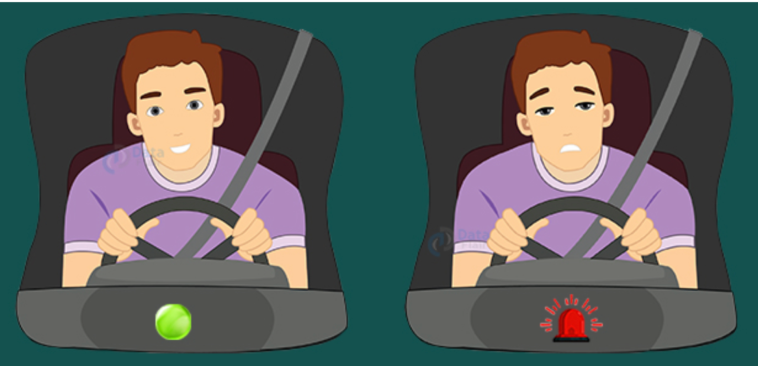
\includegraphics[width=0.40\textwidth]{Fahrer.png}
     \caption{Driver Drowsiness Detection}
\end{figure}

Die Aufgabe des Projektes stellt das Bild, 'Driver Drowsiness Detection' dar.

Auf dem Bild ist eine Person zu sehen, die in zwei unterschiedlichen Positionen hinter einem Lenkrad sitzt.

Auf dem linken Bild ist zu erkenne, dass die Person munter und entspannt hinterm dem Steuer sitzt.

Zudem zeigt eine grüne Lampe an, dass bei der linken Situation keine Probleme/Gefahren entstehen.

Auf dem rechten Bild, ist die selbe Person dargestellt, jedoch leuchtet hier eine rote Warnlampe.

Auch sieht man der Person an, dass sie müde oder angespannt ist.

Die Person hat ihre Mundwinkel nach unten gerichtet und die Augen sind leicht geschlossen.

Die Aufgabe besteht darin, zu erkennen wann die Person fahrtüchtig ist (grüne Lampe bedeutet Augen offen) oder nicht fahrtüchtig (rote Lampe bedeutet Augen geschlossen).


\subsection{Ziel}
Das Ziel des Projektes ist, zu erkennen, ob eine Person hinter dem Steuer fahrtüchtig oder nicht fahrtüchtig ist. 

Um das Ziel umzusetzen, wird ein Programm benötigt welches erkennen soll, wann die Person ihre Augen offen oder geschlossen hat.

So soll das Programm über eine 'Webcam' das Gesicht der Person erkennen und die Werte einlesen.

Mit den Werten soll entschieden werden, ob die Person weiterfahren darf oder eine Pause einlegen muss.

Dies soll über ein rotes Warnsignal und Tonsignal dem Fahrer angezeigt werden.
\newline
\newline
 \section{Diagramme}
 
Zum Start des Projektes, hielt ich alle Ideen zum Projekt, in einer Requirements Tabelle fest. 
 
 \begin{figure}[htbp]
  \centering
     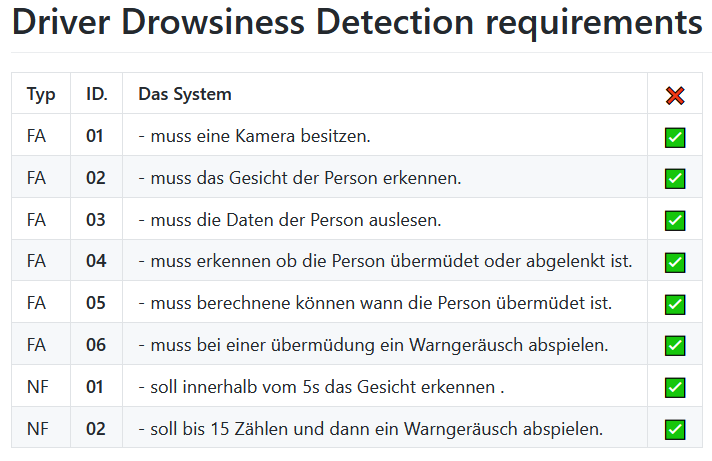
\includegraphics[width=0.48\textwidth]{DLReq.png}
     \caption{Requirements}
\end{figure}


Aus der Requirements Tabelle folgte ein Use-Case Diagramm, um den Ablauf der einzelnen Aktoren zu verdeutlichen.

\begin{figure}[htbp]
  \centering
     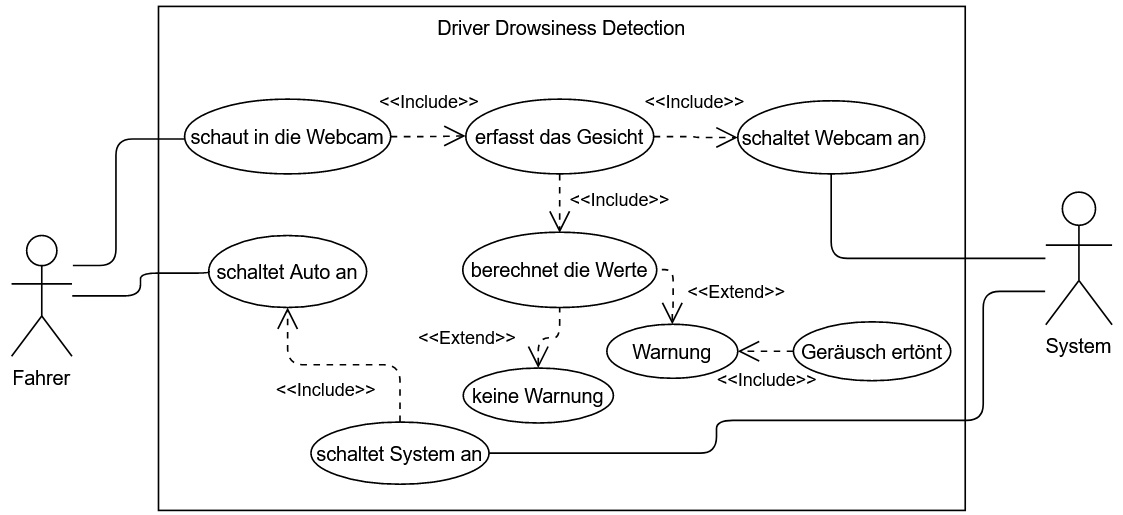
\includegraphics[width=0.48\textwidth]{UseCaseDL.png}
     \caption{Use-Case}
\end{figure}
\section{Begriffe/Beispiele}

\subsection{Begriffsbestimmung}

Als 'Driver Drowsiness Detection System', im Deutschen Aufmerksamkeits-Assistent, wird eine Müdigkeitserkennung in Kraftfahrzeugen bezeichnet.

Diese Erkennung soll helfen, Unfälle durch schläfrig werdende Fahrer oder Fahrerinnen zu vermeiden. 

Nicht nur das Einschlafen am Steuer ist gefährlich, auch die Müdigkeit reduziert die Fahrtüchtigkeit deutlich. 

Wer schläfrig fährt, schätzt die Geschwindigkeiten falsch ein. 

Man ist unkonzentriert und reagiert ähnlich langsam wie nach dem Konsum von Alkohol.

Im schlimmsten Fall nickt die Fahrerin oder der Fahrer ein. 

Mit dem System soll frühzeitig erkannt werden, ob der Fahrer übermüdet ist und so ein Unfall vermieden werden.\cite{b7}

\subsection{Beispiele}

\subsection{Mazda Mx-30}
Der 'Mazda MX-30' besitzt im Innenraum eine 
Infrarotkamera die Blickrichtung, Augen- und Mundwinkelbewegungen der Person am Steuer überwacht. 

Auch Tageszeit, Geschwindigkeit oder Blinkverhalten werden vom System berücksichtigt und ausgewertet.

Wenn die Person müde wirkt warnt das System die Person über ein akustisches Geräusch.\cite{b2}


\subsection{Andere Autos}
Die meisten Autos verfügen noch nicht über eine eingebaute Innenraum-Kamera.

Sie verwenden in ihrem Sicherheitssystem, nur die Lenkbewegungen und die Position des Fahrzeugs in der Fahrspur. 

Die Software erstellt zu Beginn der Fahrt ein Profil und analysiert das Fahrverhalten ab einer Geschwindigkeit von 65 km/h (zum Beispiel bei VW) oder 80 km/h (bei Mercedes).

Erkennt das System ein Fahrmuster, das auf die Unaufmerksamkeit des Fahrers hindeutet, wird dieser durch ein akustisches Signal oder einem visuellen Hinweis auf dem Zentraldisplay drauf hingewiesen.

Die Idee dahinter, wer am Steuer müde wird, macht öfters kleine Lenkfehler und versucht sie abrupt zu korrigieren. 

Das erkennt die Elektronik, die als Lenkwinkelsensor oftmals als Teil des 'Schleuderschutzes ESP' verbaut ist. 

Auch die Fahrtdauer, das Blinkverhalten oder die Betätigung der Pedale fließen in die Berechnung ein.\cite{b4}
\newline
\newline




 
\section{Projekt/Driver/Drowsiness/Detection/System}

Für das Projekt 'Driver Drowsiness Detection System', wird ein Programm erstellt, welches mit einer Webcam erkennen kann, ob die Person im Auto ihre Augen geöffnet oder geschlossen hat.

Falls die Augen des Fahrers oder der Fahrerin eine 
bestimmte Zeit nicht erfasst werden können, werden die Insassen des Autos mit einem Geräusch gewarnt.

\subsection{Programmierung/Installierung}

Für das Python Projekt 'Driver Drowsiness Detection System', wird das Programm 'OpenCV' benötigt. 

OpenCV ist eine Programmbibliothek mit Algorithmen für die Bildverarbeitung und Computer Vision.

Sie kann für die Programmiersprachen C, C++, Python und Java genutzt werden.

Die Bibliothek befasst sich mit der Gesichtserkennung, 3D-Funktionalität und Funktionen für die Kamerakalibrierung.

Das Deep Learning Modul von OpenCV, zum Beispiel 'YOLO', empfängt die Bilddaten und kann bis zu 80 verschiedene Objekte Identifizieren.

Mit OpenCV werden Bilder von unterschiedlichen Augen gesammelt, um diese in ein Deep Learning Model umzuwandeln, so dass später erkannt werden kann, ob die Augen von den Personen geöffnet oder geschlossen sind.

Der erste Schritt des Projekts ist es, von den verschiedenen Augen, eine Datenbank zu erstellen.

So werden mehrere tausende Bilder von Augen 
abgespeichert, zu einem 'Data Set' verpackt und daraufhin dem Programm beigebracht. 

Das Programm kann so später jegliche Augen von Personen erkennen und auslesen.   


Das Model des Projektes wird mit Keras (Convolutional Neural Networks) erstellt. 

Keras ist eine Open Source Deep-Learning Bibliothek, in der Programmiersprache Python.

Keras kann für TensorFlow, Microsoft Cognitive Toolkit und Theano genutzt werden.


Eine CNN besteht aus einem Input-, Output- und einem Hidden-Layer welche mehrere Schichten haben kann.

So wird ein Filter für die Layers genutzt um eine 2D Matrix zu erstellen. 

\newpage
Keras imports für das Projekt:
\begin{lstlisting}
from keras.preprocessing import image
from keras.utils.np_utils import to_categorical
from keras.models import Sequential
from keras.models import load_model
\end{lstlisting}

Voraussetzungen für das Projekt:
Python, Webcam, OpenCV (Gesicht/Augen Erkennung), TensorFlow (für Keras), Keras (Model) und Pygame (Sound).\cite{b1}


\subsection{Ablauf des Programmes}

\subsection{Schritt 1: Verwendung der Kamera, als Input}


Durch die Webcam werden die empfangenden Bilder als Input für das Programm verwendet. 

Über OpenCv, wird sich mit der Webcam verbunden über die Methode.
\begin{lstlisting}
Methode: cv2.VideoCapture(o) 
\end{lstlisting}

Auch muss jedes Frame, welches gespeichert wird, in einer Variable abgespeichert werden.
\begin{lstlisting}
Methode: cap.read()
\end{lstlisting}


\subsection{Schritt 2: Gesicht erkennen und eine Region of Interest (ROI) erstellen.}

Um in der Webcam das Gesicht zu erkennen, muss das Bild zu einem Grayscale umgewandelt werden, denn OpenCv arbeitet mit Grauen Images. 

Es werden keine Farben benötigt um die Gesichter zu erkennen. 

Mit der Methode 'haar cascade' wird das Gesicht der Person in der Webcam erkannt. 

\begin{lstlisting}
Methode: 

(face = cv2.CascadeClassifier / 

faces = face.detectMultiScale(gray))
\end{lstlisting}

Durch die 'haar cascade' Methoden erhält man x und y Array Werte zurück. 

Über die empfangenden Array Werte kann nun ein Rahmen zur Erkennung des Gesichtes erstellt werden. 


\subsection{Schritt 3: Im Region of Interest (ROI) die Augen erkennen.}

Genau wie im Schritt 2 wird nun auch ein ROI für die Augen erstellt. 

\begin{lstlisting}
Methode: (left_eye = leye.detectMultiscale(gray)).
\end{lstlisting}

Nun werden die Daten der Augen erfasst und ein Rahmen um die Augen erstellt, 
umso die benötigten Informationen der Augen zu auszulesen.

\begin{lstlisting}
Methode: l_eye = frame[ y : y+h, x : x+w] 
\end{lstlisting}
 
l\_eye beinhaltet nur die Daten von den Augen.

Diese Daten werden in CNN hochgeladen, so das erkannt wird ob die Augen offen oder geschlossen sind. 

Mit dem rechten Auge r\_eye wird der Ablauf wie für das linke Auge wiederholt.

\subsection{Schritt 4: Classifier soll erkennen, ob das Auge offen oder geschlossen ist}

Damit der Classifier die Augen überprüfen kann, werden die Daten in CNN hochgeladen. 

Zuvor werden die Daten noch in das richtige Format umgewandelt. 

Das Grayscale wird zu einem 24*24 Pixel Bild komprimiert. 

Nun kann das Programm auf der Webcam erkennen, ob die Person ihre Augen offen oder geschlossen hat.
\begin{lstlisting}
Augen offen  (1)

Augen geschlossen (0)
\end{lstlisting}

\subsection*{Schritt 5: Ausrechnen der Werte um zu erkennen, wann die Person unaufmerksam ist.}

Jedes Mal, wenn die Person in der Kamera ihre Augen schließt, wird ein 'Counter' hochgezählt und beim Öffnen runter gezählt. 

Erreicht der Counter den Wert 15, ertönt ein Warnsignal. 

Zudem wird der  aktuelle Wert auf dem Display angezeigt.
\begin{lstlisting}
Methode:  cv2.putText()
\end{lstlisting}

Mit dieser Methode wird der Text auf dem Display angezeigt.\cite{b1}
\newline
\newline


















\section{ShowCase}


Um das  Projekt zu starten, muss auf den Ordner 'Drowsiness detection' zugegriffen werden und die Py Datei, 'drowsiness detection.py' ausgeführt werden.

Dies geschieht alles in CMD.

\begin{lstlisting}
1. cd 'Drowsiness detection'

2. Python 'drowsiness detection.py'

\end{lstlisting}


Folgend wird in der Py Datei 'dorwsiness detection auf die Unten dargestellten Dateien zugegriffen.


\begin{figure}[htbp]
  \centering
     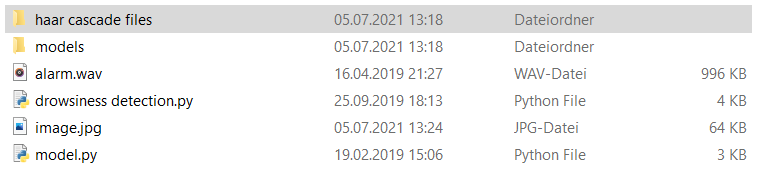
\includegraphics[width=0.48\textwidth]{Dateien.png}
     \caption{Dateien}
\end{figure}

Im 'haar cascade files', befinden sich die xml Dateien, 
die benötigt werden um die Gesichter und Augen zu erkennen.


Der 'models' Ordner enthält das model fiel 'cnn.Cat2.h5', 
für das mehrdimensionale Array im 'Convolutional neural network'. 

Zur Erkennung der Details im Bild.


Zudem beinhaltet der Ordern die 'alarm.wav' Datei,
um das Warnsignal abzuspielen, wenn der kritische Wert erreicht ist.


'Drowsiness detection' ist die Hauptdatei zum starten des Programmablaufes.


In dem Python Code, werden die einzelnen Dateien aufgerufen und ausgeführt.
\newpage
\begin{lstlisting}
model = load_model('models/cnncat2.h5')

sound = mixer.Sound('alarm.wav')


face = cv2.CascadeClassifier

('haar cascade files
\haarcascade_frontalface_alt.xml')

leye = cv2.CascadeClassifier

('haar cascade files
\haarcascade_lefteye_2splits.xml')

reye = cv2.CascadeClassifier

('haar cascade files
\haarcascade_righteye_2splits.xml')

\end{lstlisting} 

Um das das vollständige Programm zu starten.\cite{b1}

\subsection{Beispiel}

\begin{figure}[htbp]
  \centering
     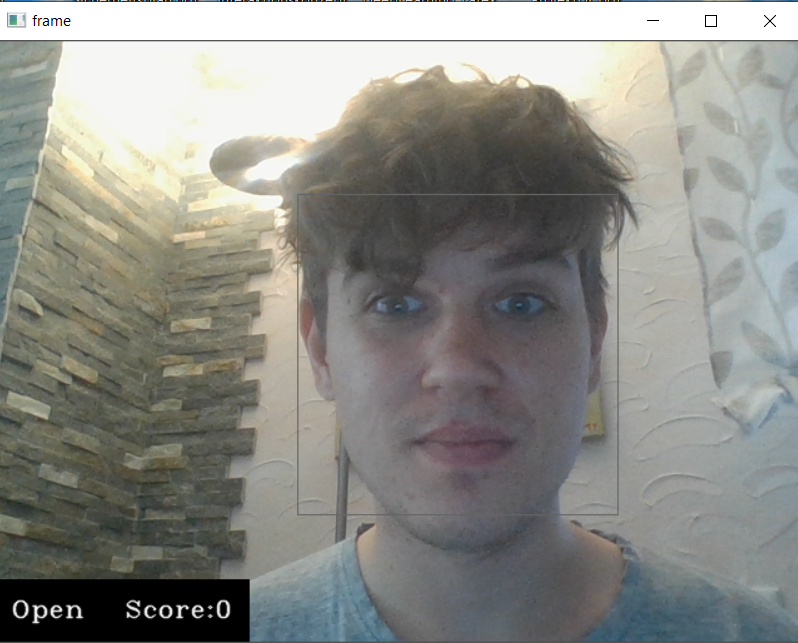
\includegraphics[width=0.35\textwidth]{Open.png}
     \caption{Open}
\end{figure}

Auf dem Bild ist zu sehen, dass das Gesicht der Person erkannt wird.

Es wird festgestellt, dass die Augen geöffnet(open) sind.

Der Score befindet sich deshalb bei '0' und sendet kein Geräusch aus.

\begin{figure}[htbp]
  \centering
     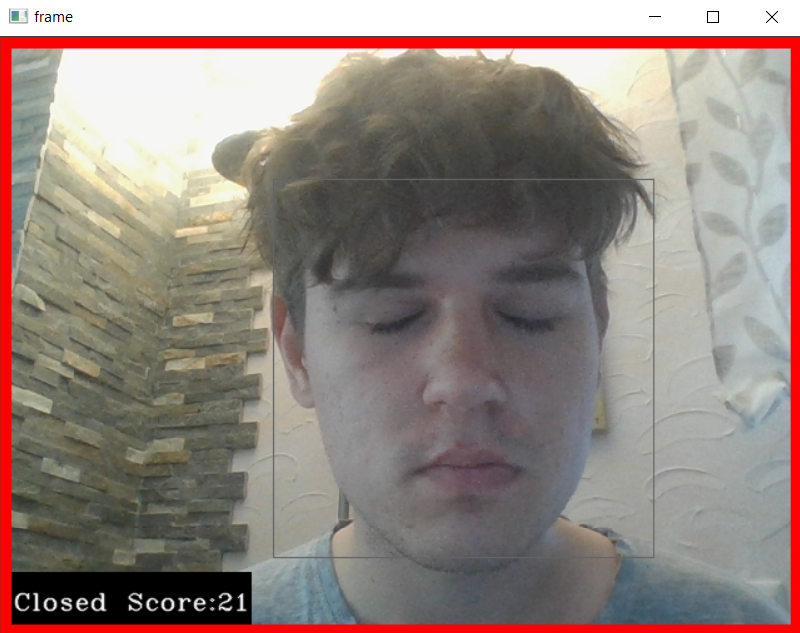
\includegraphics[width=0.35\textwidth]{Closed.png}
     \caption{Closed}
\end{figure}

Im nächsten Bild ist zu erkennen, dass die Augen der Person geschlossen (closed) sind.

So wird der Score hochgezählt und der Rand zeigt ein Warnzeichen an mit einer roten Umrandung.

Zum Schluss wird ab einem Score von '15' ein Warnsignal abgespielt.
\newline
\newline
\section{Fazit}
\subsection{Zukunft}

Das Thema Sicherheit in Autos nimmt von Jahr zu Jahr zu, bedingt durch die vielen Unfälle, die auf den Straßen passieren.

Doch nicht viele Autos sind mit einer Kamera ausgerüstet.

Die meisten Sicherheitssysteme analysieren nur das Fahrverhalten des Fahrers und zeigen ein 'Kaffee-Symbol' auf dem Display an.

Die Firma Bosch arbeitet zurzeit an einer kompletten Beobachtung des Innenraumes.

So soll bis zum Jahr 2022 ein System auf den Markt gebracht werden, die jede Person im Auto erfassen kann.

Sie erkennt, wenn Kinder auf dem Rücksitz ihren Gurt lösen und warnt den Fahrer oder die Fahrerin.

Sitzt ein Mitfahrer im Fond zu weit nach vorne gelehnt oder gar schräg und mit den Füßen auf dem Nebensitz, können Airbags und Gurtstraffer bei einem Unfall nicht schützen. 

Auch kann mit dem System verhindert werden, dass der Airbag auslöst, wenn eine Babyschale auf dem Vordersitz angebracht wird. 

Ein weiterer wichtiger Punkt für Bosch ist es, zu erfassen ob Kinder oder Tiere unabsichtlich bei sonnigen Wetter im Auto gelassen werden. 

Falls dies erkannt wird, werden sofort die Eltern oder der Rettungsdienst alarmiert.  

In der Zukunft erhofft man sich, mit den neuen Sicherheitssystemen mehr Sicherheit für die Autofahrer. 

So soll Jahr für Jahr versucht werden die Unfallrate zu verringern.\cite{b7}

\subsection{Fazit}

Zusammenfassend, ist das Thema 'Driver Drowsiness Detection System' ein wichtiger Bestandteil unseres Alltages geworden.

Nicht nur weil so verhindert werden kann, dass Personen am Steuer einschlafen,
sondern auch einige weitere Risiken wie Handys oder weiteres, welche den Fahrer ablenken könnten und so eventuell zu einem Unfall führen.

Leider sind noch nicht viele Autos mit so einem System ausgestattet.

So wie im 'Mazda Mx30' beschrieben, dass eine Kamera in Blickrichtung der fahrenden Person schaut. 

Zudem ertönt ein Signal, falls die Person müde wirkt.
 
Dieses ist heutzutage noch kein Standard in den herkömmlichen Autos. 

Es wird in den meisten Autos nur auf die Fahr- und Lenkweise des Fahrers geachtet. 

Dies wird dann nur über ein Kaffee Symbol oder über einer Nachricht auf dem Display angezeigt.

Zwar zeigt es dem Fahrer an, dass er müde sein kann, doch es hindert ihn nicht daran übermüdet weiter zu fahren.

Darum sollten mehr Autos mit dem System vom 'Mazda Mx30' ausgestattet werden, denn das Warnsignal würde den Fahrer konstant signalisieren eine Pause einzulegen.

Mit dem Projekt 'Driver Drowsiness Detection System', wurde gezeigt, dass es für viele Hersteller sehr leicht möglich ist, so ein System in ihren Autos zu implementieren.

Doch leider gibt es noch kein Gesetz, welches vorschreibt eine Kamera im Auto anbringen zu müssen.

Viele Firmen finden die Produktion von solchen Systemen nicht notwendig und arbeiten nicht mit diesem.

Viele Autobesitzer möchten eine solche Kamera nicht in ihrem Auto haben, aus Angst sie könnten überwacht werden oder abgefilmt.

Auch wegen der vielen Gesetze, ist es den Firmen oft nicht möglich Kameras in öffentlichen Räumen zu installieren.

Die Firma Bosch versucht trotz der schwierigen Lage, so ein System im Jahr 2022 zu veröffentlichen.

Zusätzlich zu der Kamera, die auf den Fahrer gerichtet ist, möchten sie auch die anderen Insassen beobachten.

Diese können sich im Auto auch in einer Notlage befinden und der Notruf soll daraufhin gewählt werden oder der Halter des Autos informiert werden.


Schluss folgend ist das Thema 'Driver Drowsiness Detection System', noch nicht ausgreift. 

Da es noch zu viele negative Punkte gibt, die verhindern, dass jeder Autobesitzer so ein System in seinem Auto installieren möchte.\cite{b7}









\newpage




\begin{thebibliography}{00}

\bibitem{b1} https://data-flair.training/blogs/python-project-driver-drowsiness-detection-system/

\bibitem{b2} https://smartrider.ch/de/aktuelles/muedigkeit-am-steuer-ist-gefaehrlich

\bibitem{b3} https://www.aachener-zeitung.de/ratgeber/auto/fahrassistenzsysteme

\bibitem{b4} https://www.bussgeldkatalog.org/muedigkeitserkennung/

\bibitem{b5} https://ysjournal.com/medical-image-translation-using-convolutional-neural-networks/

\bibitem{b6} https://www.tt.com/artikel/18188598/uebermuedung-am-steuer-2020-ursache-fuer-268-unfaelle

\bibitem{b7} https://www.bosch-presse.de/pressportal/de/de/lebensretter-per-kamera-mit-bosch-behaelt-das-auto-seine-insassen-im-blick-204288


\end{thebibliography}
\vspace{12pt}
\end{document}